\chapter{Numerical Calculus}
In this brief chapter we discuss techniques for approximating the two primary computations
in calculus: taking derivatives and evaluating definite integrals. Throughout this chapter
we will make heavy use of Taylor's Theorem to build these approximations. 


\section{Numerical Differentiation}
In this section we'll build several approximation of first and second derivatives.  The
idea for each of these approximation is:
\begin{itemize}
    \item Partition the interval $[a,b]$ into $N$ points.
    \item Approximate the derivative at the point $x \in [a,b]$ by using linear
        combinations of $f(x-h)$, $f(x)$, $f(x+h)$, and/or other points in the partition.  
\end{itemize}
Partitioning the interval into discrete points turns the continuous problem of finding a
derivative at every real point in $[a,b]$ into a discrete
problem where we calculate the approximate derivative at finitely many points in $[a,b]$.
Figure \ref{fig:differentiation_partition} shows a depiction of the partition as well as
making clear that $h$ is the separation between each of the points in the partition.  Note
that in general the points in the partition do not need to be equally spaced, but that is
the simplest place to start.
\begin{figure}[ht!]
    \begin{center}
        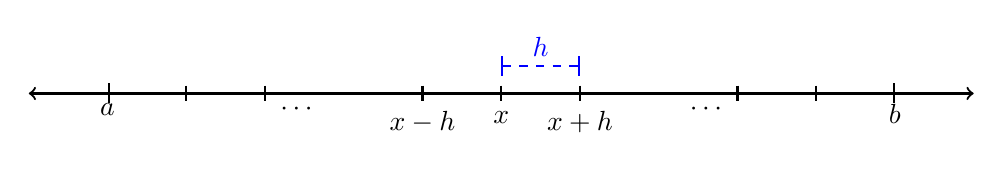
\begin{tikzpicture}
            \draw[<->, thick] (-1,0) -- (11,0);
            \draw[|-|,thick] (0,0) node[anchor=north]{$a$} -- (10,0)
            node[anchor=north]{$b$};
            \foreach \j in {1,2,8,9}{
                \draw[thick] (\j,0.1) -- (\j,-0.1);
            }
            \draw (2.4,0) node[anchor=north]{$\cdots$};
            \draw (7.6,0) node[anchor=north]{$\cdots$};
            \draw[thick] (4.0,0.1) -- (4,-0.1) node[anchor=north]{$x-h$};
            \draw[thick] (5,0.1) -- (5,-0.1) node[anchor=north]{$x$};
            \draw[thick] (6.0,0.1) -- (6,-0.1) node[anchor=north]{$x+h$};
            \draw[dashed, blue, thick,|-|] (5,0.35) -- (6,0.35);
            \draw[blue] (5.5,0.35) node[anchor=south]{$h$};
        \end{tikzpicture}
    \end{center}
    \caption{A partition of an interval on the real line.}
    \label{fig:differentiation_partition}
\end{figure}

If we recall that the definition of the first derivative of a function is
\begin{flalign}
    \frac{df}{dx} = \lim_{h \to 0} \frac{f(x+h) - f(x)}{h}.
    \label{eqn:derivative_defintiion}
\end{flalign}
our first approximation for the first derivative is naturally
\begin{flalign}
    \frac{df}{dx} \approx \frac{f(x+h) - f(x)}{h}.
    \label{eqn:derivative_first_approx}
\end{flalign}
In \eqref{eqn:derivative_first_approx} we have simply removed the limit and instead
approximated the derivative as the slope.  It should be clear that this approximation is
only good if $h$ is {\it small}.  The linear combination that we
spoke about before is
\[ \frac{df}{dx} \approx \frac{1}{h} f(x+h) - \frac{1}{h} f(x). \]
While this is the simplest and most obvious approximation for the first derivative there
is a much more elegant technique, using Taylor series, for arriving at this approximation.
Furthermore, the Taylor series technique suggests an infinite family of other techniques.


\begin{problem}\label{prob:numdiff1}
    From Taylor's Theorem we know that for an infinitely differentiable function $f(x)$,
    \[ f(x) = f(a) + \frac{f'(a)}{1!} (x-a)^1 + \frac{f''(a)}{2!}(x-a)^2 +
        \frac{f^{(3)}(a)}{3!}(x-a)^3 + \frac{f^{(4)}(a)}{4!}(x-a)^4 + \cdots. \] 
    What do we get if we replace $x$ with $x+h$ and $a$ with $x$?  In other words, in
    Figure \ref{fig:differentiation_partition} we want to center the Taylor series at $x$
    and evaluate the resulting series at the point $x+h$.
\end{problem}


\begin{problem}\label{prob:num_diff_first_order}
    Solve the result from the previous problem for $f'(x)$ to create an approximation for
    $f'(x)$ using $f(x+h)$, $f(x)$, and some higher order terms.  How can we use Taylor's
    Theorem to quantify the error of this approximation?
\end{problem}
\solution{
    \begin{flalign*}
        f(x+h) &= f(x) + \frac{f'(x)}{1!}(x+h-x) + \frac{f''(x)}{2!}h^2 + \cdots \\
        f'(x) &= \frac{f(x+h)-f(x)}{h} + \frac{f''(\xi)}{2} h \quad \text{for} \quad \xi
        \in (x,x+h)
    \end{flalign*}
    The error is on the order of $h$.
}

\begin{definition}[Order of a Numerical Derivative]
    The {\bf order} of a numerical derivative is the power of the step size in the
    remainder term.  For example, a first order method will have ``$h^1$'' in the
    remainder term.  A second order method will have ``$h^2$'' in the reaminder term.
\end{definition}

\begin{thm}[First Order Approximation of the First
    Derivative]\label{thm:first_order_first_deriv}
    In problem \ref{prob:num_diff_first_order} we derived a first order approximation of
    the first derivative:
    \[ f'(x) = \frac{f(x+h) - f(x)}{h} + \mathcal{O}(h). \]
    In this formula, $h = \Delta x$ is the step size.
\end{thm}
In the previous definition, ``$\mathcal{O}(h)$'' (read: big-O of $h$) states that the
method is first order.  This means that the maximum error that you're making with this
method is on the order of the size of the step.  Not surprisingly, if we let $h$ get
arbitrarily small then the error in this method gets arbitrarily small.  More formally we
have the following definition.

\begin{definition}[Big $\mathcal{O}$ Notation]
    We say that the error in a differentiation method is ``big O of $h$'', $E =
    \mathcal{O}(h)$, if and only if there is a positive constant $M$ such that 
    \[ |Error| \le M |h|. \]
    This is equivalent to saying that a differentiation method is first order.
\end{definition}

\begin{problem}
    Explain what the phrase
    \begin{quote}
        {\it ``The approximation of $f'(x)$ in Theorem \ref{thm:first_order_first_deriv} is $\mathcal{O}(h)$''}
    \end{quote}
    into your own words.  
\end{problem}

\begin{problem}
    Writet MATLAB code that takes a function and a domain $(xmin,xmax)$ and
    returns a numerical approximation to the derivative on the interval
    $(xmin,xmax)$. Your function should accept an anonymous function handle, the
    bounds on the domain, and the number of interior points used for approximation within
    the domain.  Your function should output the $x$ values and $y$ values associated with
    the derivative.\\
    \mcode{function [new_x,dfdx]=FirstDerivFirstOrder(f,xmin,xmax,num_interior_pts)} 
\end{problem}

The only two ways to really check a numerical derivative is to plot the numerical
approximation and to do the derivative by hand and to plot the error. Be warned, however,
that the numerical derivative that we have built from Theorem
\ref{thm:first_order_first_deriv} should have one less value than the
original list of $x$ and $y$ values.  Think about why this must be true. Also double check
your code from the previous problem and make sure that you can plot \mcode{new_x} vs
\mcode{dfdx} without having to change their size.  

\begin{problem}
    Write a MATLAB script that find a first order approximation for the first derivative
    of $f(x) = \sin(x) - x\sin(x)$ on the interval $x \in (0,15)$.  Your script should
    output two plots (side-by-side). 
    \begin{enumerate}
        \item The left-hand plot should show the function in blue and the first derivative
            as a red dashed curve. Sample code for this problem is
    \begin{lstlisting}
     f = @(x) sin(x) - x*sin(x);
     a=0; b=15;
     num_interior_pts = 1000; % this should be LARGE
     x = linspace(a,b,num_interior_pts);
     [new_x,dfdx] = FirstDerivFirstOrder(f,a,b,num_interior_pts);
     subplot(1,2,1)
     plot(x, f(x) , 'b' , new_x , dfdx , 'r--')
    \end{lstlisting}
        \item The right-hand plot should show the absolute error between the exact derivative and
            the numerical derivative.
    \begin{lstlisting}
    df = @(x) ... % write code for the exact derivative
    subplot(1,2,2)
    plot(new_x, abs( df(new_x) - dfdx ) , 'k--')
    \end{lstlisting}
    \end{enumerate}
    Discuss how you can see the fact that this is a first order method.
\end{problem}


% \begin{problem}\label{prob:numdiff2}
%     Write Excel and MATLAB code that takes a data set from an
%     unknown function and returns a first-order accurate numerical approximation of the
%     first derivative of the function. Test your code on data gerenated from the function
%     \[ f(x) = \sin(x) - x\sin(x) \quad \text{on} \quad x \in (0,15) \]
%     with various step sizes. Provide a plot of the error between the analytic derivative
%     and the numerical derivative using a semi-logy scale.
%     \\Note: You will lose some information along the way (why?).
% 
%     Your MATLAB code should accept the 
% \end{problem}

\begin{problem}\label{prob:numdiff3}
    Consider again the Taylor series for an infinitely differentiable function $f(x)$:
    \[ f(x) = f(a) + \frac{f'(a)}{1!} (x-a)^1 + \frac{f''(a)}{2!}(x-a)^2 +
        \frac{f^{(3)}(a)}{3!}(x-a)^3 + \frac{f^{(4)}(a)}{4!}(x-a)^4 + \cdots \] 
    This time, replace $x$ with $x-h$ and $a$ with $x$ and simplify.  Once you have the
    Taylor series centered at $x$ and evaluated at $x-h$ form the linear combination
    \[ f(x+h) - f(x-h) \]
    using your result from \ref{prob:numdiff1} and solve for $f'(x)$.  Your result should
    be a second-order accurate approximation for the first derivative of $f$.  Simplify
    your approximation formula and verify that it is indeed second order.
\end{problem}

\begin{thm}[Second Order Approximation of the First Derivative]
    \[ f'(x) = \underline{\hspace{2in}} + \mathcal{O}(h^2) \]
\end{thm}
\solution{
    Subtract the two Taylor representations to get the second order approximation.
    \begin{flalign*}
        f(x+h) &= f(x) + \frac{f'(x)}{1!}h + \frac{f''(x)}{2!}h^2 +
        \frac{f'''(x)}{3!} h^3 + \cdots \\
        f(x-h) &= f(x) - \frac{f'(x)}{1!}h + \frac{f''(x)}{2!}h^2 - \frac{f'''(x)}{3!}h^3 \cdots \\
        f(x+h)-f(x-h) &= 2 h f'(x) + \frac{h^3}{6} (f'''(\xi)+f'''(\nu)) \quad \text{for} \quad \xi
        \in (x,x+h) \quad \text{and} \quad \xi \in (x-h,x) \\
        \implies f'(x) &= \frac{f(x+h)-f(x-h)}{2h} + \frac{h^2}{12} (f'''(\xi)+f'''(\nu)) \quad \text{for} \quad \xi
        \in (x,x+h) \quad \text{and} \quad \xi \in (x-h,x) 
    \end{flalign*}
    Hence, 
    \[ f'(x) \approx \frac{f(x+h) - f(x-h)}{2h} + \mathcal{O}(h^2). \]
}

% \begin{problem}
%     Write Excel and MATLAB code that takes a data set from an unknown function and returns
%     a second-order accurate numerical approximation for the first derivative.  Test your
%     code on data generated by $f(x) = \sin(x) - x\sin(x)$ and
%     provide error plots that compare your first- and second-order accurate differentiation
%     code.
% \end{problem}
% \solution{
%     Subtract the two Taylor representations to get the second order approximation.
%     \begin{flalign*}
%         f(x+h) &= f(x) + \frac{f'(x)}{1!}h + \frac{f''(x)}{2!}h^2 +
%         \frac{f'''(x)}{3!} h^3 + \cdots \\
%         f(x-h) &= f(x) - \frac{f'(x)}{1!}h + \frac{f''(x)}{2!}h^2 - \frac{f'''(x)}{3!}h^3 \cdots \\
%         f(x+h)-f(x-h) &= 2 h f'(x) + \frac{h^3}{6} (f'''(\xi)+f'''(\nu)) \quad \text{for} \quad \xi
%         \in (x,x+h) \quad \text{and} \quad \xi \in (x-h,x) \\
%         \implies f'(x) &= \frac{f(x+h)-f(x-h)}{2h} + \frac{h^2}{12} (f'''(\xi)+f'''(\nu)) \quad \text{for} \quad \xi
%         \in (x,x+h) \quad \text{and} \quad \xi \in (x-h,x) 
%     \end{flalign*}
% }

\begin{problem}
    Write a MATLAB function that takes a function and a domain and returns a second order
    numerical approximation to the first derivative on the interval.  Your function should
    accept an anonymous function handle, the bounds on the domain, and the number of
    interior points used for approximation within the domain. Your function should output
    the x values and y values associated with the derivative.\\
    \mcode{function [new_x,dfdx]=FirstDerivSecondOrder(f,xmin,xmax,num_interior_pts)}
\end{problem}


\begin{problem}
    Add the Taylor series for $f(x+h)$ and $f(x-h)$ to arrive at an approximation of the
    second derivative. What is the order of the error?  
\end{problem}

\begin{problem}
    Write a MATLAB function that takes a function and a domain and returns a second order
    numerical approximation to the second derivative on the interval.  Your function should
    accept an anonymous function handle, the bounds on the domain, and the number of
    interior points used for approximation within the domain. Your function should output
    the x values and y values associated with the derivative.\\
    \mcode{function [new_x,ddfdxx]=SecondDerivSecondOrder(f,xmin,xmax,num_interior_pts)}
\end{problem}

\begin{problem}
    Test your second derivative code on the function $f(x) = \sin(x) - x\sin(x)$.  Create
    an error plot showing the accuracy of the method.
\end{problem}

Table \ref{tab:first_and_second_derivatives} summarizes the formulas that we have for
derivatives thus far. The exercises at the end of this chapter contain several more
derivative approximations.  We will return to this idea when we study numerical
differential equations in Chapter \ref{ch:odes}.
\begin{table}
    \centering
    \begin{tabular}{|c|c|c|c|}
        \hline
        Derivative & Formula & Error & Name \\ \hline \hline
        $1^{st}$ & $\ds f'(x) \approx \frac{f(x+h) - f(x)}{h}$ & $\mathcal{O}(h)$ & Forward
        Difference \\ \hline
        $1^{st}$ & $\ds f'(x) \approx \frac{f(x) - f(x-h)}{h}$ & $\mathcal{O}(h)$ & Backward
        Difference \\ \hline
        $1^{st}$ & $\ds f'(x) \approx \frac{f(x+h) - f(x-h)}{2h}$ & $\mathcal{O}(h^2)$ &
        Centered Difference \\ \hline
        $2^{nd}$ & $\ds f''(x) \approx \frac{f(x+h) - 2f(x) + f(x-h)}{h^2}$ &
        $\mathcal{O}(h^2)$ & Centered Difference \\ \hline
    \end{tabular}
    \caption{First and second derivatives.}
    \label{tab:first_and_second_derivatives}
\end{table}


% \begin{problem}
%     Go to the \href{http://apps.who.int/gho/data/?theme=home}{World Health Organization
%     Data Repository} and find a data set where it would make physical sense to take a
%     first or a second derivative (and that the derivative would tell you something
%     meaningful about the data).  Use your MATLAB code to take the derivative and provide
%     plots as well as context and meaning associated with the plot.  You will need to
%     download the data as a CSV or Excel file and import the proper columns into Excel
%     (Google \texttt{xlsread} to learn how MATLAB imports Excel data). Your data set will
%     obviously involved some noise, but one thought might be to find a data set that shows
%     a trend in time.
% \end{problem}


\section{Numerical Integration}
Next we will build methods for approximating integrals.  Recall that the definition of the
Riemann integral is
\begin{flalign}
    \int_a^b f(x) dx = \lim_{\Delta x \to 0} \sum_{j=1}^N f(x_j) \Delta x
    \label{eqn:Riemann_integral}
\end{flalign}
where $N$ is the number of subintervals on the interval $[a,b]$ and $\Delta x$ is the
width of the interval.  As with differentiation, we can remove the limit and have a decent
approximation of the integral
\[ \int_a^b f(x) dx \approx \sum_{j=1}^N f(x_j) \Delta x. \]
You are likely familiar with this approximation of the integral from Calculus. The value of $x_j$ can
be chosen anywhere within the subinterval and three common choices are to use the left
endpoint, the midpoint, and the right endpoint.  We see
a depiction of this in Figure \ref{fig:integral_with_rectangles}.  

\begin{figure}[ht!]
    \begin{center}
        \begin{tikzpicture}[x=1.5cm, line cap=round, line join=round] 
            \foreach \k [count=\z] in {0, 1/4, 1/2}{
                \begin{scope}[shift=(0:\z*3)]
                    \path [plot fill] plot [domain=0:2] (\x,{y(\x)}) -| cycle;
                    \foreach \x in {0, 1/2, 1, 3/2}
                    \path [bar]  (\x,0) |- (\x+1/2, {y(\x+\k)}) |- cycle;
                    \path [plot]  plot [domain=0:2] (\x,{y(\x)});
                    \path [axis] (0,4.5) |- (2.5,0);
                    \foreach \t [count=\x from 0] in {0,\frac{1}{2},1,\frac{3}{2},2}
                    \path [axis, -] (\x/2,0) -- ++(0,-3pt) node [below] {$\t$};
                    \foreach \y in {0,4}
                    \path [axis, -] (0,\y) -- ++(-3pt, 0) node [left] {$\y$};
                    \foreach \x in {0, 1/2, 1, 3/2}
                    \path [marking]  (\x+\k, {y(\x+\k)}) circle [radius=1.5pt];
                \end{scope}
            }
        \end{tikzpicture}
    \end{center}
    \caption{Riemann sum to approximate an integral with left, midpoint, and right
    rectangles.}
    \label{fig:integral_with_rectangles}
\end{figure}

Clearly, the more rectangles we choose the closer the sum of the areas of the rectangles will get to the integral.
\begin{problem}
    Write MATLAB code approximate an integral withe Riemann sums.  Your MATLAB function
    should accept an anonymous function handle, a lower bound, an upper bound, the number
    of subintervals, and an optional input that allows the user to designate whether they
    want left, right, or midpoint rectangles. \\
    \mcode{function Area=MyRiemannSum(f, a, b, num_subintervals, type)} \\
    Test your code on several functions for which you know the integral.
\end{problem}

\begin{problem}
    Create a plot with the width of the subintervals on the horizontal axis and the
    absolute error between your (left) Riemann sum calculation and the exact integral for
    a known definite integral.  Your plot should be on a log-log scale.  Based on your
    plot, what is the approximate order of the error in the Riemann sum approximation?
\end{problem}

\begin{problem}
    We want to approximate $\displaystyle \int_a^b f(x) dx$.  One of the simplest ways is
    to approximate the area under the function with a trapezoid.  Recall from basic
    geometry that area of a
    trapezoid is $A = \frac{1}{2} (b_1 + b_2) h$.  In terms of the integration problem we
    can do the following:
    \begin{enumerate}
        \item First partition $[a,b]$ into the set $\{x_0=a, x_1, x_2, \ldots, x_{n-1},
        x_n=b\}$.
        \item On each part of the partition approximate the area with a trapezoid:
            \[ A_j = \frac{1}{2} \left[ f(x_j) + f(x_{j-1}) \right]\left(
            x_j - x_{j-1} \right) \]
        \item Approximate the integral as
            \[ \int_a^b f(x) dx = \sum_{j=1}^n A_j \]
    \end{enumerate}
    Draw a picture depicting how the trapezoidal rule works.
\end{problem}

The trapezoidal rule does a decent job approximating integrals, but ultimately you are
using linear functions to approximate $f(x)$ and the accuracy may suffer if the step
size is too large or the function too non-linear. You likely notice that the trapezoidal
rule will give an exact answer if you were to integrate a linear or constant function. A
potentially better approach would be to get an integral that evaluates quadratic functions
exactly. In order to do this we need to evaluate the function at three points (not two
like the trapezoidal rule). Let's integrate a function $f(x)$ on the interval
$[a,b]$ by using the three points $(a,f(a))$, $(m,f(m))$, and
$(b,f(b))$ where $m=\frac{a+b}{2}$ is the midpoint of the two boundary points. We want to
find constants $A1$, $A2$, and $A3$ such that the integral
\[ \int_a^b f(x) dx = A_1 f(a) + A_2 f\left( \frac{a+b}{2} \right) + A_3 f(b) \]
is exact for all constant, linear, and quadratic functions. This would guarantee that we
have an exact method for all polynomials of order 2 or less but should serve as a decent
approximation if the function is not quadratic.

To find the constants $A_1, A_2$, and $A_3$ we can write the following system of three
equations
\begin{flalign*}
    \int_a^b 1 dx &= b-a = A_1 + A_2 + A_3 \\
    \int_a^b x dx &= \frac{b^2 - a^2}{2} = A_1 a + A_2 \left( \frac{a+b}{2} \right) + A_3
    b \\
    \int_a^b x^2 dx &= \frac{b^3 - a^3}{3} = A_1 a^2 + A_2 \left( \frac{a+b}{2} \right)^2
    + A_3 b^2.
\end{flalign*}
Solving the linear system gives
\[ A_1 = \frac{b-a}{6}, \quad A_2 = \frac{4(b-a)}{6}, \quad \text{and} \quad
A_3 = \frac{b-a}{6}. \]
At this point we can see that the integral can be approximated as
\[ \int_a^b f(x) dx \approx \left( \frac{b-a}{6} \right) \left( f(a) + 4f\left(
    \frac{a+b}{2}
\right) + f(b) \right) \]
and the technique will give an exact answer for any polynomial of order 2 or below.  To
improve upon this idea we now examine the problem of partitioning the interval $[a,b]$
into small pieces and running this process on each piece.



\begin{problem}
    Now we put the process explained above into a form that can be coded to approximate
    integrals. We call this method Simpson's Rule after Thomas Simpson (1710-1761) who, by
    the way, was a basket weaver in his day job so he could pay the bills and keep doing
    math.
    \begin{enumerate}
        \item First parition $[a,b]$ into the set $\{x_0=a, x_1, x_2, \ldots, x_{n-1},
        x_n=b\}$.
        \item On each part of the partition approximate the area with a parabola:
            \[ A_j = \frac{1}{6} \left[ f(x_j) + 4 f\left( \frac{x_j+x_{j-1}}{2} \right) +
                f(x_{j-1}) \right]\left( x_j - x_{j-1} \right) \]
        \item Approximate the integral as
            \[ \int_a^b f(x) dx = \sum_{j=1}^n A_j \]
    \end{enumerate}
    Draw a picture depicting how the trapezoidal rule works.
\end{problem}

\begin{problem}
    Write MATLAB functions that implement both the trapezoidal rule and Simpson's rule.
    Keep in mind that MATLAB deals with vectors and iteration in very nice ways.  You
    shouldn't need a \texttt{for loop} in your function.

    Test both MATLAB functions on known integrals and approximate the order of the error
    based on the mesh size.  
\end{problem}


Thus far we have three numerical approximations for definite integrals: Riemann sums (with
rectangles), the trapezoidal rule, and Simpsons's rule.  There are MANY other
approximations for integrals and we leave the further research to the curious reader.
\begin{thm}[Numerical Integration Techniques]
    Let $f(x)$ be a continuous function on the interval $[a,b]$.  The integral $\int_a^b
    f(x) dx$ can be approximated with any of the following.
    \begin{flalign*}
       &\text{Riemann Sum: }  \int_a^b f(x) dx \approx \sum_{j=1}^N f(x_j) \Delta x \\
       &\text{Trapezoidal Rule: }  \int_a^b f(x) dx \approx \frac{1}{2} \sum_{j=1}^N
       \left( f(x_j) + f(x_{j-1}) \right) \Delta x \\
       &\text{Simpson's Rule: }  \int_a^b f(x) dx \approx \frac{1}{6} \sum_{j=1}^N \left(
       f(x_j) + 4 f\left( \frac{x_j + x_{j-1}}{2} \right) + f(x_{j-1}) \right) \Delta x \\
    \end{flalign*}
    where $\Delta x = x_j - x_{j-1}$ and $N$ is the number of subintervals.
\end{thm}


\section{Exercises}
\begin{problem}
    {\bf Coding Challenge:} The four adjacent digits in the 1000-digit number that have
    the greatest product are $9 \times 9 \times 8 \times 9 = 5832$.

    \begin{center}
    73167176531330624919225119674426574742355349194934\\
    96983520312774506326239578318016984801869478851843\\
    85861560789112949495459501737958331952853208805511\\
    12540698747158523863050715693290963295227443043557\\
    66896648950445244523161731856403098711121722383113\\
    62229893423380308135336276614282806444486645238749\\
    30358907296290491560440772390713810515859307960866\\
    70172427121883998797908792274921901699720888093776\\
    65727333001053367881220235421809751254540594752243\\
    52584907711670556013604839586446706324415722155397\\
    53697817977846174064955149290862569321978468622482\\
    83972241375657056057490261407972968652414535100474\\
    82166370484403199890008895243450658541227588666881\\
    16427171479924442928230863465674813919123162824586\\
    17866458359124566529476545682848912883142607690042\\
    24219022671055626321111109370544217506941658960408\\
    07198403850962455444362981230987879927244284909188\\
    84580156166097919133875499200524063689912560717606\\
    05886116467109405077541002256983155200055935729725\\
    71636269561882670428252483600823257530420752963450
\end{center}

    Write code to find the thirteen adjacent digits in the 1000-digit number that have the
    greatest product. What is the value of this product?
\end{problem}
\solution{%Source: Project Euler Problem \#8: Solution: 
23514624000}


\begin{problem}
    {\bf Coding Challenge:} 2520 is the smallest number that can be divided by each of the
    numbers from 1 to 10 without any remainder.  Write code to find the smallest positive
    number that is evenly divisible by all of the numbers from 1 to 20?
\end{problem}
\solution{% Source: Project Euler Problem \#5: Solution: 
232792560 }

\begin{problem}
    For each of the following numerical differentiation formulas (1) prove that the
    formula is true, and (2) find the order of the method. To prove that each of the
    formulas is true you will need to write the Taylor series for all of the terms in the
    numerator on the right and then simplify to solve for the necessary derivative.  The
    highest power of the remainder should reveal the order of the method.
    \begin{enumerate}
        \item[(a)] $\ds f'(x) \approx \frac{\frac{1}{12} f(x-2h) - \frac{2}{3} f(x-h) +
            \frac{2}{3} f(x+h) - \frac{1}{12} f(x+2h)}{h}$
        \item[(b)] $\ds f'(x) \approx \frac{-\frac{3}{2} f(x) + 2 f(x+2) -
            \frac{1}{2} f(x+h)}{h}$
        \item[(c)] $\ds f''(x) \approx \frac{-\frac{1}{12} f(x-2h) + \frac{4}{3} f(x-h) -
            \frac{5}{2} f(x) + \frac{4}{3} f(x+h) - \frac{1}{12} f(x+2h)}{h^2}$
        \item[(d)] $\ds f'''(x) \approx \frac{-\frac{1}{2} f(x-2h) + f(x-h) - f(x+h) +
            \frac{1}{2} f(x+2h)}{h^3}$
    \end{enumerate}
\end{problem}

\begin{problem}\label{prob:first_deriv_data}
    Write a MATLAB function that accepts a list of $(x,y)$ ordered pairs from an Excel
    spreadsheet and returns a list of $(x,y)$ ordered pairs for a first order
    approximation of the first derivative of the
    underlying function. \\
    \mcode{function [new_x,dydx] = FirstDeriveFromData(ExcelFileName,Xrange,Yrange)} \\
    In the function all of the inputs are strings.  For example \\
    \mcode{FirstDerivativeFromData('MyFunctionData.xlsx','A2:A101','B2:B101')}\\
    Create a test Excel file and a test script that have graphical output showing that
    your MATLAB function is finding the correct derivative.
\end{problem}




\begin{problem}
    Write a MATLAB function that accepts a list of $(x,y)$ ordered pairs from an Excel
    spreadsheet and returns a list of $(x,y)$ ordered pairs for a second order
    approximation of the second derivative of the
    underlying function. \\
    \mcode{function [new_x,dydx] = SecondDeriveFromData(ExcelFileName,Xrange,Yrange)} \\
    In the function all of the inputs are strings.  For example \\
    \mcode{SecondDerivativeFromData('MyFunctionData.xlsx','A2:A101','B2:B101')}\\
    Create a test Excel file and a test script that have graphical output showing that
    your MATLAB function is finding the correct derivative.
\end{problem}


\begin{problem}\label{prob:trap_from_data}
    Write a MATLAB function that implements the trapezoidal rule on a list of $(x,y)$
    order pairs representing the integrand function.  The list of ordered pairs should be
    read from an Excel file. \\
    \mcode{function Area = TrapezoidFromData(ExcelFilename, Xlist, Ylist)}\\
    In the function all of the inputs are strings.  For example \\
    \mcode{Area = TrapezoidFromData('MyFunctionData.xlsx','A2:A101','B2:B101')}\\
    Create a test Excel file and a test script showing that your MATLAB function is
    finding the correct integral.
\end{problem}

\begin{problem}
    Use numerical integration to answre the question in each of the following scenarios
    \begin{enumerate}
        \item[(a)] We measure the rate at which water is flowing out of a reservoir (in
            gallons per second) several times over the course of one hour.  Estimate the
            total amount of water which left the reservoir during that hour.
            \begin{center}
                \begin{tabular}{|l||c|c|c|c|c|c|c|}
                    \hline
                    time (min) & 0 & 7 & 19 & 25 & 38 & 47 & 55 \\ \hline
                    flow rate (gal/sec) & 316 & 309 & 296 & 298 & 305 & 314 & 322 \\ \hline
                \end{tabular}
            \end{center}
        \item[(b)] The department of transportation finds that the rate at which cars
            cross a bridge can be approximated by the fucntion
            \[ f(t) = \frac{22.8 \text{cars/min}}{3.5 + 7(t-1.25)^4}, \]
            where $t=0$ at 4pm, and is measured in hours.  Estimate the total number of
            cars that cross the bridge betwee 4 and 6pm.  Make sure that your estimate has
            an error less than 5\%.
    \end{enumerate}
\end{problem}


\begin{problem}
    Consider the integrals 
    \[ \int_{-2}^2 e^{-x^2/2} dx \quad \text{and} \quad \int_0^1 \cos(x^2) dx. \]
    Neither of these integrals have closed-form solutions so a numerical method is
    necessary.  Create a loglog plot that shows the errors for the integrals with different values of $h$ (log
    of $h$ on the $x$-axis and log of the error on the $y$-axis).
    Write a complete interpretation of the loglog plot.  
    To get the {\it exact} answer for these plots use the MATLAB \mcode{quad} command.
    (What we're really doing here is comparing our algorithms to MATLAB's algorithm).
\end{problem}


\begin{problem}
    Go to \href{https://www.data.gov/}{data.gov} or the
    \href{http://apps.who.int/gho/data/?theme=home}{World Health Organization Data
    Repository} and find data sets for the following tasks.
    \begin{enumerate}
        \item[(a)] Find a data set where the variables naturally lead to a meaningful
            derivative.  Use your code from Problem  \ref{prob:first_deriv_data} to
            evaluate and plot the derivative.  If your data appears to be subject to
            significant noise then use the Excel curve fitting tools first to smooth the
            data; then do the derivative.  Write a few sentences explaning what the
            derivative means in the context of the data.
        \item[(b)] Find a data set where the variables naturally lead to a meaningfun
            definite integral.  Use your code from Problem \ref{prob:trap_from_data} to
            evaluate the definite integral.  If your data appears to be subject to
            significant noise then use the Excel curve fitting tools first to smooth the
            data; then do the integral.  Write a few sentences explaning what the
            integral means in the context of the data.
    \end{enumerate}
    In both of these tasks be very cautious of the units on the data sets and the units of
    your answer. 
\end{problem}

% \begin{problem}
%     Go to the \href{http://apps.who.int/gho/data/?theme=home}{World Health Organization
%     Data Repository} and find a data set where it would make physical sense to integrate
%     (and that the integral would tell you something meaningful about the data).  Use your
%     MATLAB code to take the integral and provide context and meaning associated with the
%     integral.  You will need to download the data as a CSV or Excel file and import the
%     proper columns into Excel (Google \texttt{xlsread} to learn how MATLAB imports Excel
%     data). Your data set will obviously involved some noise, but one thought might be to
%     find a data set that shows a trend in time.
% \end{problem}



\begin{problem}
    Go to the USGS water data repository: \\
    \href{https://maps.waterdata.usgs.gov/mapper/index.html}{https://maps.waterdata.usgs.gov/mapper/index.html}.\\
    Here you'll find a map with information about water resources around the country.
    \begin{itemize}
        \item Zoom in to a dam of your choice (make sure that it is a dam).
        \item Click on the map tag then click ``Access Data''
        \item From the dropdown menu at the top select either ``Daily Data'' or ``Current
            / Historical Data''.  If these options don't appear then choose a different
            dam.
        \item Change the dates so you have the past year's worth of information.
        \item Select ``Tab-separated'' under ``Output format'' and press Go.  Be sure that
            the data you got has a flow rate (ft$^3$/sec).
        \item At this point you should have access to the entire data set.  Copy it into a
            \texttt{csv} file and save it to your computer.
    \end{itemize}
    For the data that you just downloaded you have three tasks: (1) plot the data in a
    reasonable way giving appropriate units, (2) find the total amount of water that
    has been discharged from the dam during the past calendar year, and (3) report any
    margin of error in your calculation based on the numerical method that you used in
    part (2).
\end{problem}


\begin{problem}
    Integrate each of the functions over the interval $[-1,2]$ and verify mathematically
    that your numerical integral is correct to 10 decimal places.  Then provide a plot of
    the function along with its numerical first derivative.
    \begin{enumerate}
        \item[(a)] $\ds f(x) = \frac{x}{1+x^4}$
        \item[(b)] $\ds g(x) = (x_1)^3 (x-2)^2$
        \item[(c)] $\ds h(x) = \sin\left(x^2\right)$
    \end{enumerate}
\end{problem}


\begin{problem}
    Although Simpson’s rule was derived from parabolas, prove that it integrates all cubic
    polynomials exactly.
\end{problem}
